\documentclass[12pt]{article}
 
\usepackage[margin=1in]{geometry} 
\usepackage{amsmath,amsthm,amssymb}
\usepackage{graphicx}
\usepackage{tikz}
\usepackage{wrapfig}
\usetikzlibrary{calc,patterns,angles,quotes}
 
\newcommand{\N}{\mathbb{N}}
\newcommand{\Z}{\mathbb{Z}}
\newcommand{\R}{\mathbb{R}}
\newcommand{\C}{\mathbb{C}}

\usepackage{mathtools}

\DeclarePairedDelimiter\ceil{\left\lceil}{\right\rceil}
\DeclarePairedDelimiter\floor{\left\lfloor}{\right\rfloor}
 
\usepackage{amsthm}
\newtheorem{proposition}{Proposition}
\newtheorem{question}{Question}
 
\begin{document}
 
% --------------------------------------------------------------
%                         Start here
% --------------------------------------------------------------
 
\title{Solutions to Exercise Sheet 1}
\author{Leif Van Holland \\ \\
\textsc{Discrete and Computational Geometry}}

\maketitle

\section*{Exercise 1}
\begin{proposition}[upper bound]
Let $\Gamma$ be the set of non-intersecting polygonal chains $C$ in the plane where the geometric dilation $\delta(C)>1$. Let $n$ be the number of vertices of $C$ and $P(C)$ be the number of pairs $p,q\in C$, where the geometric dilation of $C$ is attained and $p$ is a vertex of $C$. Then
\[P(C)\in O(n^2) \text{ if } C\in\Gamma.\]
\end{proposition}
\begin{proof}
From Lemma 2 we know, that for every pair $p,q\in C$ where $C$ attains maximum dilation, at least one of the points has to be a vertex of $C$. W.l.o.g., let $p$ be a vertex of $C$. Using the method described in the lecture, we can determine the maximum dilation of $C$ for every vertex-edge-pair $p,e$ by parameterizing $e$ as points $q(t)\in e, t\in I$ with $|I|=|e|$. This yields the following equation
\[\delta(p,q(t)) = \frac{t+|C_p^q|}{r(t)},\qquad r(t) := \sqrt{t^2-2\cos\beta|pq|t+|pq|^2} \]
and its derivative with respect to t
\begin{align}\delta'(p,q(t)) = \frac{r(t)-\frac{1}{2r(t)}(2t-2\cos\beta|pq|)(t+|C_p^q|)}{r(t)^2}.
\label{deltaderiv}
\end{align}
Roots of \eqref{deltaderiv} provide points $q(t)$ that maximize the dilation of $C$. We can see with
\begin{align*}
    0 = \delta'(p,q(t))
    \iff 0 = t^2 - 2 \cos\beta |pq|t+|pq|^2-\frac{1}{2}(2t-2\cos\beta|pq|)(t+|C_p^q|), 
\end{align*}
that \eqref{deltaderiv} has at most two roots $t_1, t_2$. Therefore, every of the $n\cdot(n-1)$ vertex-edge-pairs contributes at most two pairs $(p,q(t_1))$ and $(p,q(t_2))$, where maximum dilation of $C$ is attained. In other words
\[
P(C) < 2\cdot n(n-1) \in O(n^2)
\]
\end{proof}

\begin{proposition}[lower bound] Let $C\in\Gamma$. Then the following statement holds
\[P(C) \in \Omega(n^2).\]
\end{proposition}
\begin{proof}
We prove this by giving a construction scheme for a chain $C=(p_1, ..., p_n), n\geq2$. In the following, $e_1\perp e_2$ denotes that two line segments $e_1, e_2$ are perpendicular.
\begin{itemize}
    \item For $i=1$, choose any $p_1\in\R^2$.
    \item For $i=2$, choose any $p_2\in\R^2$ with $|C_{p_1}^{p_2}| = 1$.
    \item For $i=3$, choose $p_3\in\R^2$ so that $C_{p_1}^{p_2} \perp C_{p_2}^{p_3}$ and $|C_{p_2}^{p_3}| = 1$
    \item For $i>3$, choose $p_i\in\R^2$ so that $C_{p_{i-2}}^{p_{i-1}} \perp C_{p_{i-1}}^{p_i}, |p_{i-2}p_i| = |p_{i-3}p_{i-1}|$ and $|C_{p_{i-1}}^{p_i}| = 1$.
\end{itemize}
Following this scheme, $C$ might looks as follows:

\begin{figure}[h]
\centering
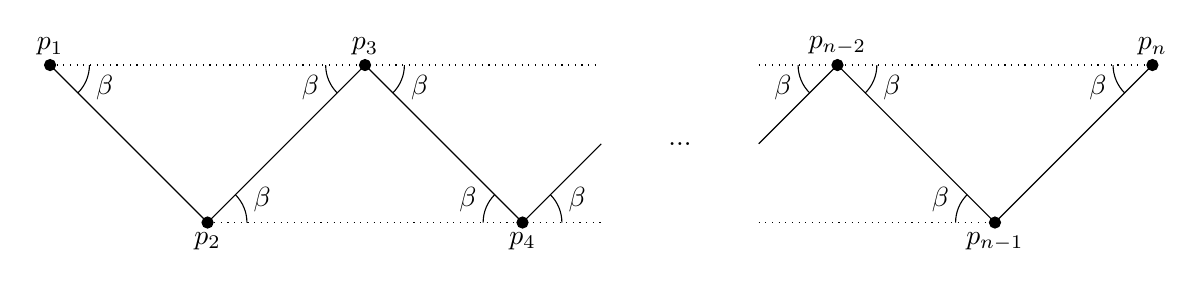
\begin{tikzpicture}

\coordinate (p1) at (0,0);
\coordinate (p2) at (2,-2);
\coordinate (p3) at (4,0);
\coordinate (p4) at (6,-2);
\coordinate (p4a) at (7,-1);
\coordinate (pn2a) at (9,-1);
\coordinate (pn2) at (10,0);
\coordinate (pn1) at (12,-2);
\coordinate (pn) at (14,0);

\draw (p1) -- (p2) -- (p3) -- (p4) -- (p4a);

\filldraw[black] (p1) circle (2pt) node[anchor=south] {$p_1$};
\pic [draw, -, "$\beta$", angle eccentricity=1.5] {angle = p2--p1--p3};

\filldraw[black] (p2) circle (2pt) node[anchor=north] {$p_2$};
\pic [draw, -, "$\beta$", angle eccentricity=1.5] {angle = p4--p2--p3};

\filldraw[black] (p3) circle (2pt) node[anchor=south] {$p_3$};
\pic [draw, -, "$\beta$", angle eccentricity=1.5] {angle = p4--p3--pn2};
\pic [draw, -, "$\beta$", angle eccentricity=1.5] {angle = p1--p3--p2};

\filldraw[black] (p4) circle (2pt) node[anchor=north] {$p_4$};
\pic [draw, -, "$\beta$", angle eccentricity=1.5] {angle = p3--p4--p2};
\pic [draw, -, "$\beta$", angle eccentricity=1.5] {angle = pn1--p4--p4a};

\node at (8,-1) {...};
\draw (pn2a) -- (pn2) -- (pn1) -- (pn);

\filldraw[black] (pn2) circle (2pt) node[anchor=south] {$p_{n-2}$};
\pic [draw, -, "$\beta$", angle eccentricity=1.5] {angle = p3--pn2--pn2a};
\pic [draw, -, "$\beta$", angle eccentricity=1.5] {angle = pn1--pn2--pn};

\filldraw[black] (pn1) circle (2pt) node[anchor=north] {$p_{n-1}$};
\pic [draw, -, "$\beta$", angle eccentricity=1.5] {angle = pn2--pn1--p4};

\filldraw[black] (pn) circle (2pt) node[anchor=south] {$p_n$};
\pic [draw, -, "$\beta$", angle eccentricity=1.5] {angle = pn2--pn--pn1};

\draw[dotted] (p1) -- (7,0);
\draw[dotted] (9,0) -- (pn);
\draw[dotted] (p2) -- (7,-2);
\draw[dotted] (9,-2) -- (pn1);
\end{tikzpicture}
\end{figure}

Observe that this construction causes all vertices with odd indices to lie on a line segment $l_{odd}$ and all vertices with even indices to lie on another line $l_{even}$. From Lemma 1 we know that
\begin{align}
    C \text{ attains a locally maximal dilation at } p,q\in C \iff \cos \beta = \frac{-|pq|}{|C_p^q|}
    \label{localcondition}
\end{align}
where $\beta$ is the angle enclosed by the edge $e\in C$ with $p\in e$ that is on the path to $q$ and the line segment $pq$. W.l.o.g. we will only consider vertices with an odd index for now (the construction is completely analogous for even indices). All these vertices lie on the line segment $l_{odd}$. Let $p_i, p_j$ be two of these vertices and w.l.o.g $i<j$. Let $\beta$ be the angle defined like above.

From the construction scheme we can derive that
\begin{itemize}
    \item[(i)] $|p_i p_{i+1}| = |p_{i+1}p_{i+2}| = 1$,
    \item[(ii)] $p_i, p_{i+1}, p_{i+2}$ form a triangle $T$ where ($p_i p_{i+1} \perp p_{i+1}p_{i+2}$), $p_i p_{i+2}$ is the hypotenuse of $T$ with length $|p_i p_{i+2}| = \sqrt{2}$ and is a subsegment of $l_{odd}$,
    \item[(iii)] $\beta \overset{\text{(ii)}}{=} \frac{\pi}{4}$,
    \item[(iv)] $|p_i p_j| = \sqrt{2}\cdot\left(\frac{j-i}{2}\right)$ and $|C_{p_i}^{p_j}| = j-i$
\end{itemize}
From these observations we can conclude that
\[\frac{-|p_i p_j|}{|C_{p_i}^{p_j}|}\overset{\text{(iv)}}{=}\frac{-\sqrt{2}\cdot\frac{1}{2}(j-i)}{(j-i)} = -\frac{1}{\sqrt{2}} = \cos\frac{\pi}{4} \overset{\text{(iii)}}{=} \cos{\beta}.  \]
From \eqref{localcondition} we now know that the dilation is locally maximal and this result was obtained regardless of the choice of $i$ and $j$. Therefore we get
\[ \delta(p_i,p_j) = \delta(C) = \sqrt{2} \text{ for all odd vertex indices } i,j.\]
We can repeat this argument with even indices and get the same result. This means that for every vertex $p\in C$, we find $(\floor{\frac{n}{2}}-1)$ other vertices $p_j$ with $\delta(C) = \delta(p_i,p_j) = \sqrt{2}$. In total, this amounts to
\[ P(C) = n\cdot\left(\floor{\frac{n}{2}}-1\right) \in \Omega(n^2) \]
\end{proof}

\begin{proposition}
If $C\not\in\Gamma$ is an arbitrary non-intersecting polygonal chain, then $P(C) = \infty$.
\end{proposition}
\begin{proof} 
By definition, $C\not\in\Gamma$ implies that $\delta(C)\leq 1$. Because for all $p,q\in C$, $|C_p^q| \geq |pq|$ always holds, we can conclude that
\[\delta(C)=\max_{\substack{p,q\in C\\p\neq q}} \frac{|C_p^q|}{|pq|}=1\]
and more specifically
\[\forall p,q\in C, p\neq q: \delta_C(p,q) = \delta(C) = 1.\]
There is an infinite amount of choices for $p$ and $q$, therefore \[P(C) = \infty.\]
\end{proof}

\section*{Exercise 2}

\begin{proposition}
It exists a planar graph $G$, where the maximum graph-theoretic dilation of $G$ is attained by a pair of non-visible vertices.
\end{proposition}

\begin{wrapfigure}{r}{0.25\textwidth}
    \centering
    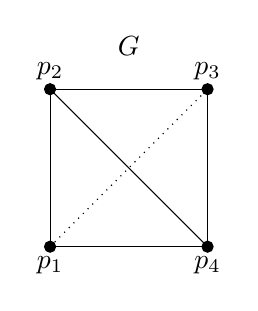
\begin{tikzpicture}
    \coordinate (p1) at (0,0);
    \coordinate (p2) at (0,2);
    \coordinate (p3) at (2,2);
    \coordinate (p4) at (2,0);
    
    \draw (p2) -- (p1) -- (p4) -- (p3);
    \draw (p2) -- (p3) node[midway, above=0.3cm] {$G$};
    \draw (p2) -- (p4);
    \draw[dotted] (p1) -- (p3);
    \filldraw[black] (p1) circle (2pt) node[anchor=north] {$p_1$};
    \filldraw[black] (p2) circle (2pt) node[anchor=south] {$p_2$};
    \filldraw[black] (p3) circle (2pt) node[anchor=south] {$p_3$};
    \filldraw[black] (p4) circle (2pt) node[anchor=north] {$p_4$};
    
    \end{tikzpicture}
\end{wrapfigure}
\leavevmode

\begin{proof}
Let $G$ be the graph shown on the right with $|p_1p_2| = |p_2p_3| = |p_3p_4| = |p_4p_1| = 1$. To determine the maximum dilation, we calculate the dilation for all six pairs $p_i, p_j, i<j$. As all but one pair of vertices are adjacent to one another, we get the trivial values
\[ \delta(p_1,p_2) = \delta(p_2,p_3) = \delta(p_3,p_4) = \delta(p_1,p_4) = \delta(p_2,p_4) = 1 \]
and for the remaining pair
\[ \delta(p_1, p_3) = \frac{|\pi_{p_1}^{p_3}|}{|p_1p_3|} = \frac{2}{\sqrt{2}} = \sqrt{2} \: \text{ with } \: \pi_{p_1}^{p_3} = (p_1, p_2, p_3). \]
So in fact, $\delta(G) = \delta(p_1,p_3)$ and $p_1, p_3$ are not co-visible, as the line segment $p_1p_3$ is intersected by $p_2p_4$.
\end{proof}

\begin{proposition}
Let $G$ be a planar, simply connected graph. There is always a pair of points $p,q\in G$ with maximal (geometric) dilation $\delta(G)$ so that $p$ and $q$ are co-visible.
\end{proposition}

\begin{proof}
The argument to prove this proposition is very similar to Lemma 3 from the lecture. Assume $p,q\in G$ are two  non-visible points with $\delta(p,q) = \delta(G)$. Let $q'\in G$ be a point where an edge of $G$ intersects the line segment $pq$ and w.l.o.g. $p,q'$ and $q',q$ are co-visible. Let $\pi_p^q$ denote the shortest path between $p$ and $q$ in $G$. Then
\begin{align}
    \delta(G) = \frac{|\pi_p^q|}{|pq|} = \frac{|\pi_p^q|}{|pq'|+|q'q|} \overset{(*)}{\leq} \frac{|\pi_p^{q'}|+|\pi_{q'}^q|}{|pq'|+|q'q|} \leq \max\left\{ \frac{|\pi_p^{q'}|}{|pq'|}, \frac{|\pi_{q'}^q|}{|q'q|}\right\} \overset{(**)}{\leq} \delta(G)
    \label{sandwich}
\end{align}
${\scriptstyle(*)}\: |\pi_p^q| \leq |\pi_p^{q'}|+|\pi_{q'}^q|$ always holds, because for $\pi_p^q$ being a shortest path between $p$ and $q$, either $q'\in\pi_p^q \implies |\pi_p^q|=|\pi_p^{q'}|+|\pi_{q'}^q|$ or we have to make a detour to get to $q'$ before getting to $q$, which implies $|\pi_p^q|<|\pi_p^{q'}|+|\pi_{q'}^q|$. ${\scriptstyle(**)}$ also holds, as $\delta(G)$ is defined to be the maximum dilation of $G$. With \eqref{sandwich} we can conclude that $\delta(p,q')=\frac{|\pi_p^{q'}|}{|pq'|} = \delta(G)$ or $\delta(q',q)=\frac{|\pi_{q'}^q|}{|q'q|} = \delta(G)$. Both of these pairs are co-visible.
\end{proof}

\section*{Exercise 3}
\begin{question}
Why do we trace the chain $p_i, p_{i+1},...,p_n$ through the additively weighted Voronoi diagram of $p_1, p_2, ..., p_i$ with weights $a_{p_i}$?
\end{question}
We trace the chain, because for every vertex $p_i$ and for every segment $s\in C \cap \text{AVR}(p_i)$ we have to determine if there is a point $q\in s$ that is below the cone $K_{p_i}$. It is not sufficient to check individual points $q$, as there are infinitely many choices for $q > p_i$.
\begin{question}
Why is it not necessary to incrementally compute the Voronoi diagrams for $p_1, p_2, ..., p_n$ and successively trace the chains $p_i, p_{i+1},...,p_n$?
\end{question}
It is sufficient to compute the Voronoi diagram only once, because it is only dependent on the constant values $|C_{p_1}^{p_i}| for 1 < i \leq n$, that we can precompute in $O(n)$. Together with the coordinates $p_i$ and $a_{p_i} = \frac{|C_{p_1}^{p_i}|}{\kappa}$, all values needed to compute the AVD are already determined. We do not require any intermediate results from the trace of the chain.

% --------------------------------------------------------------
%     You don't have to mess with anything below this line.
% --------------------------------------------------------------
 
\end{document}